% Section 9 - written by M5 (Ambrish Chauraiya). All numbers come from results/summary.csv
% through report/generated/*.tex (analysis/tables.py); none are typed by hand.
\section{Results and Analysis}
Both methods ran every experiment in Table~\ref{tab:scen}, 42 runs in total. Tables~\ref{tab:e1}--\ref{tab:e6} and Figures~\ref{fig:e1}--\ref{fig:e6} are generated directly from the logged telemetry.

\subsection{E1: altitude step response}
Figure~\ref{fig:e1} and Table~\ref{tab:e1} show the altitude response. Method A has no integral term, so it settles \R{E1}{baseline}{step2_ss_error_m}\,m below the target in both steps. The hover speed it assumes (68.5\,rad/s, taken from the sample) is slightly lower than the true hover speed, and nothing corrects for that. Because of this offset it never enters the $\pm2\,\%$ band, so its settling time is undefined. Method B's integral term removes the offset: its steady-state error is \R{E1}{improved}{step2_ss_error_m}\,m. On the 2\,m $\to$ 1\,m step its overshoot is \R{E1}{improved}{step2_overshoot_pct}\,\%, against \R{E1}{baseline}{step2_overshoot_pct}\,\% for Method A. Method B rises more slowly (\R{E1}{improved}{step1_rise_time_s}\,s against \R{E1}{baseline}{step1_rise_time_s}\,s at take-off). This is deliberate: it follows a smooth reference rather than the raw step.

\begin{figure}[H]
\centering
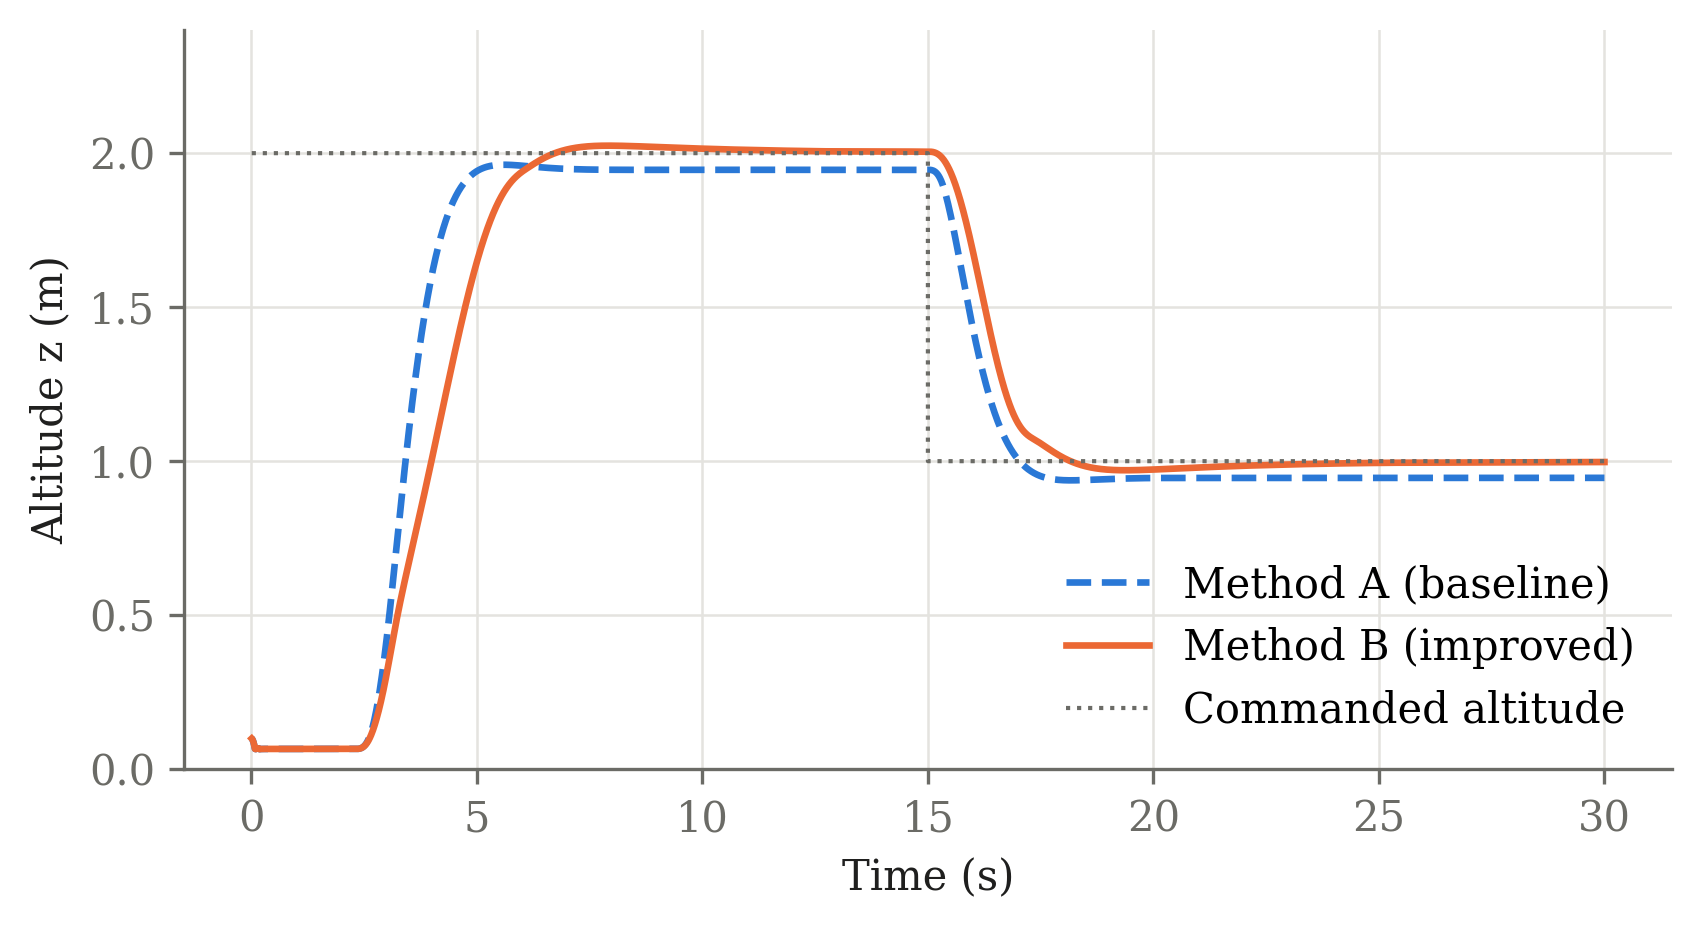
\includegraphics[width=0.62\linewidth]{fig_e1_step_response.png}
\caption{E1 altitude step response (true altitude)}
\label{fig:e1}
\end{figure}

\begin{table}[h]
\centering
\caption{E1 altitude step response (true altitude)}
\label{tab:e1}
\begin{tabular}{|p{8.2cm}|c|c|}
\hline
\textbf{Metric} & \textbf{Method A} & \textbf{Method B} \\ \hline
Take-off 0.1 m $\to$ 2.0 m: Rise time 10--90\% (s) & 1.50 & 2.41 \\ \hline
Take-off 0.1 m $\to$ 2.0 m: Overshoot (\%) & 0.0 & 1.3 \\ \hline
Take-off 0.1 m $\to$ 2.0 m: Settling time, 2\% band (s) & -- & 6.2 \\ \hline
Take-off 0.1 m $\to$ 2.0 m: Steady-state error (m) & 0.054 & 0.005 \\ \hline
Step 2.0 m $\to$ 1.0 m: Rise time 10--90\% (s) & 1.30 & 1.50 \\ \hline
Step 2.0 m $\to$ 1.0 m: Overshoot (\%) & 6.2 & 2.9 \\ \hline
Step 2.0 m $\to$ 1.0 m: Settling time, 2\% band (s) & -- & 6.1 \\ \hline
Step 2.0 m $\to$ 1.0 m: Steady-state error (m) & 0.054 & 0.003 \\ \hline
\end{tabular}
\end{table}


\subsection{E2 and E3: waypoint missions}
On the square mission (Figure~\ref{fig:e2}) both methods reach all five waypoints. Method A's path RMSE is \R{E2}{baseline}{path_rmse_m}\,m and Method B's \R{E2}{improved}{path_rmse_m}\,m (Table~\ref{tab:e2e3}). The larger differences are in how the drone is driven. Method A sees every new waypoint as a 2\,m step and immediately commands the full tilt limit. Figure~\ref{fig:tilt} shows its tilt spikes at each corner, peaking at \R{E2}{baseline}{max_tilt_deg}$^\circ$ against \R{E2}{improved}{max_tilt_deg}$^\circ$. Method B's control effort is \R{E2}{reduction}{control_effort}\,\% lower, and it finishes the mission sooner (\R{E2}{improved}{mission_time_s}\,s against \R{E2}{baseline}{mission_time_s}\,s). On the 3D mission (Figure~\ref{fig:e3}) the gap is larger. Method A's altitude offset and step commands give a path RMSE of \R{E3}{baseline}{path_rmse_m}\,m, against \R{E3}{improved}{path_rmse_m}\,m for Method B, an \R{E3}{reduction}{path_rmse_m}\,\% reduction.

\begin{figure}[H]
\centering
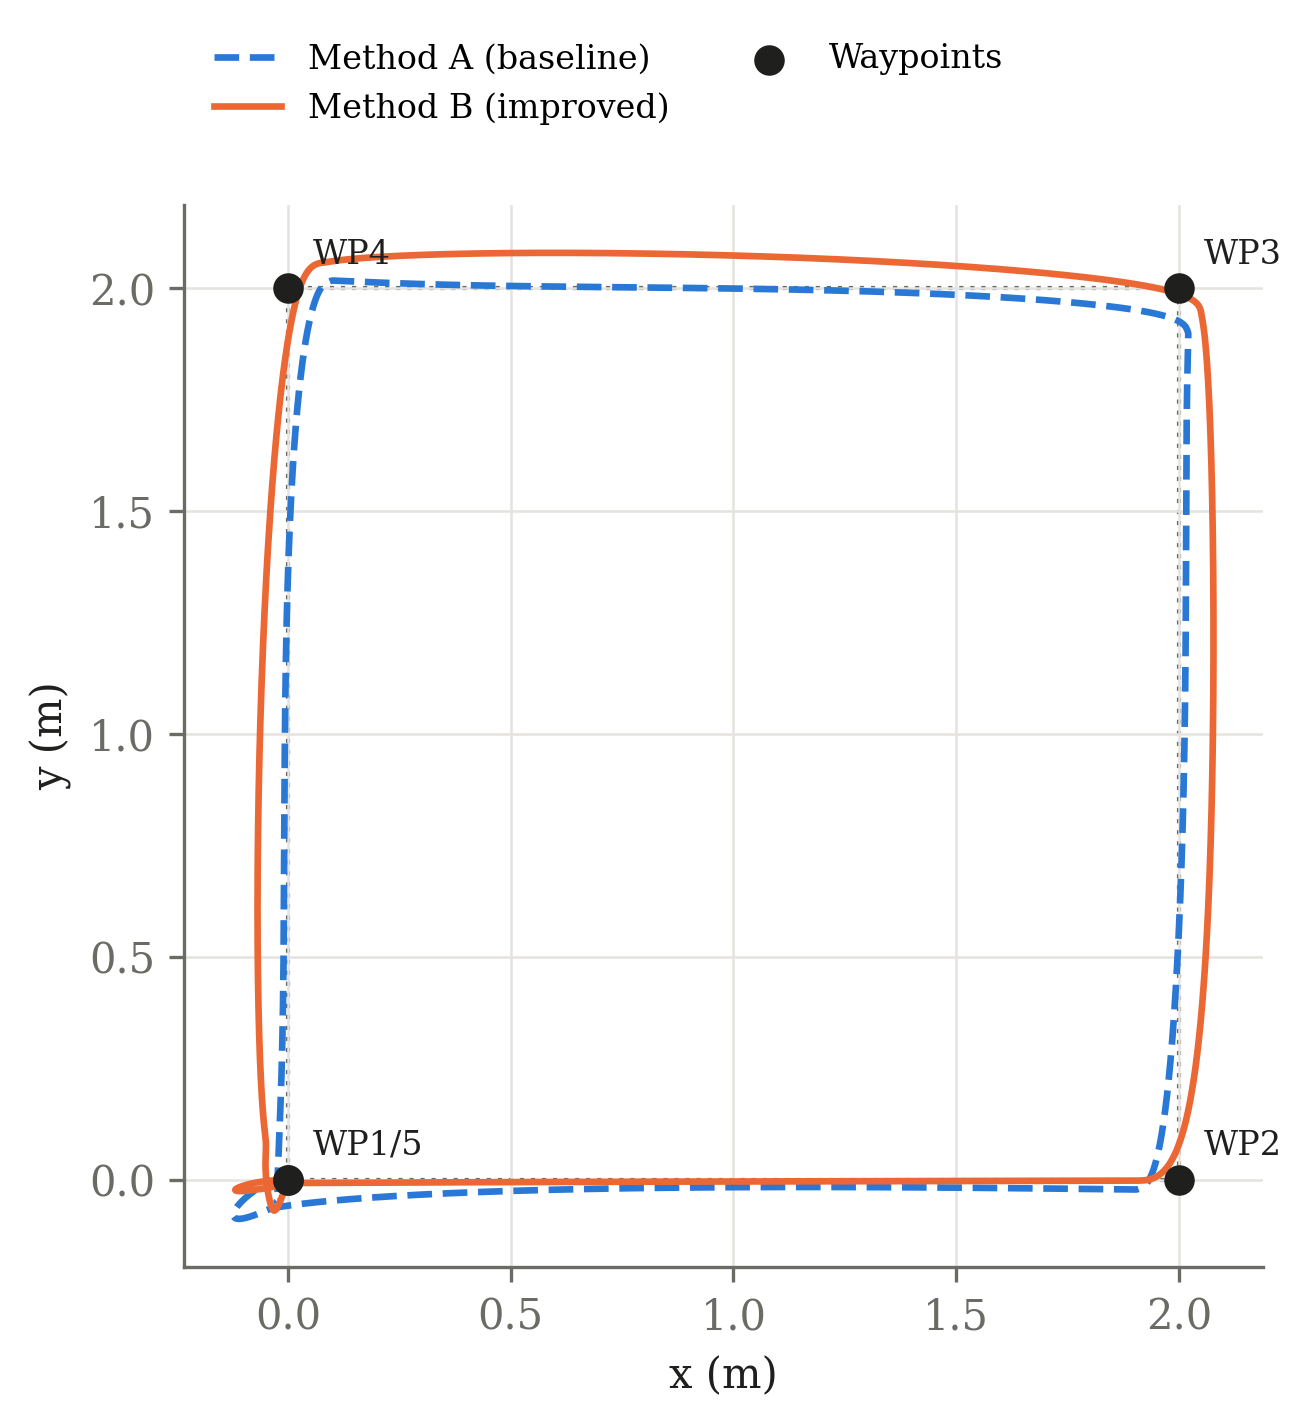
\includegraphics[width=0.45\linewidth]{fig_e2_xy_path.png}
\caption{E2 square mission, top view}
\label{fig:e2}
\end{figure}

\begin{figure}[H]
\centering
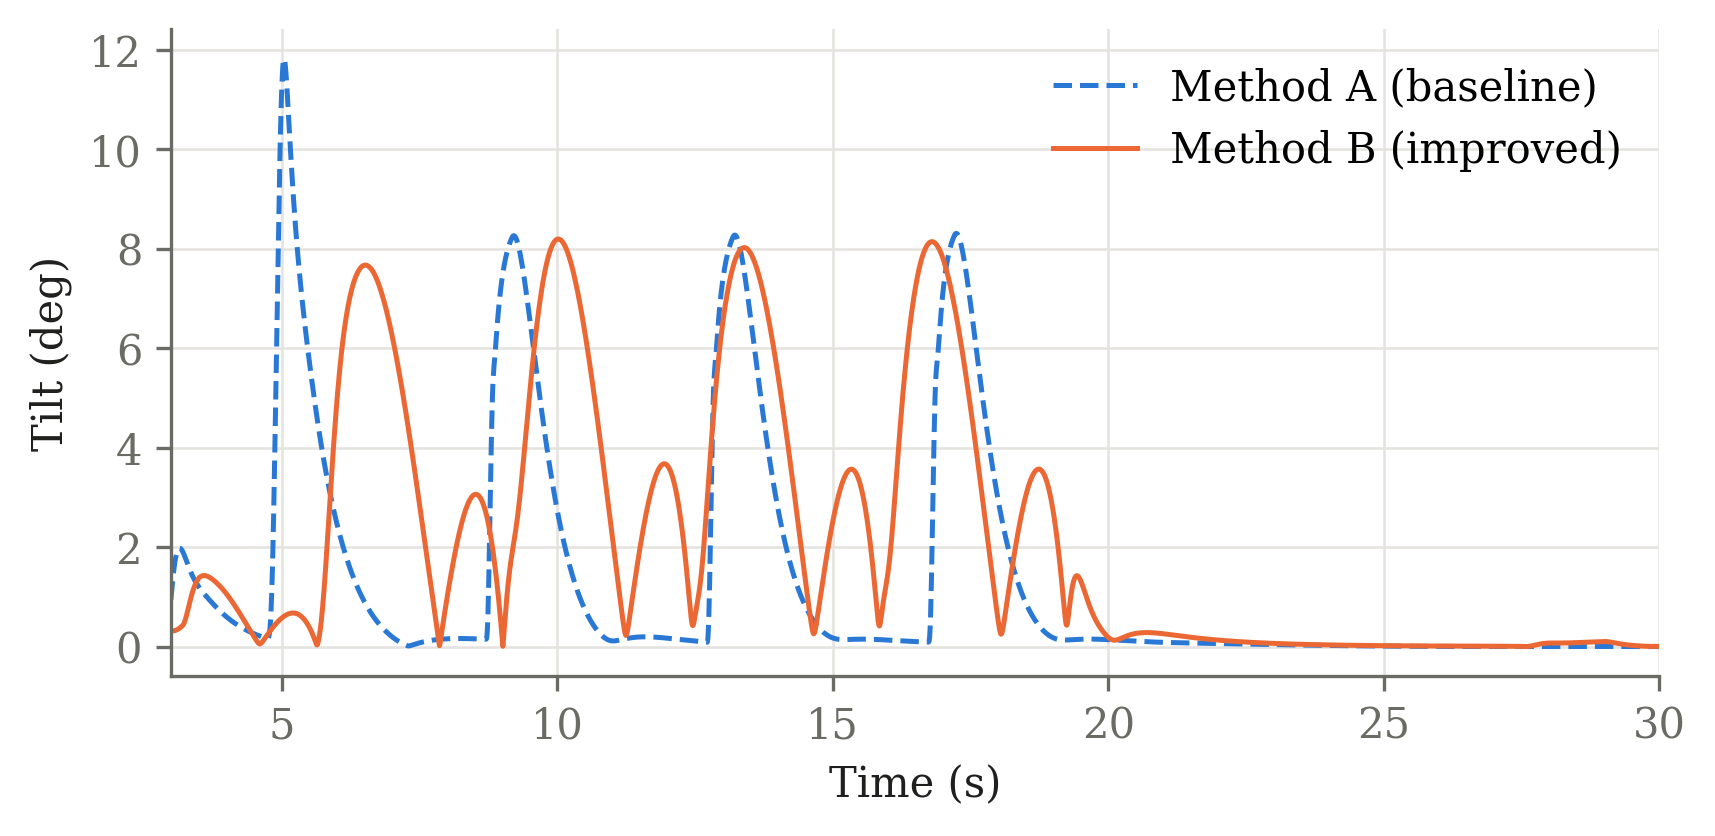
\includegraphics[width=0.62\linewidth]{fig_e2_tilt.png}
\caption{E2 tilt angle over time: step commands cause tilt spikes at each corner}
\label{fig:tilt}
\end{figure}

\begin{figure}[H]
\centering
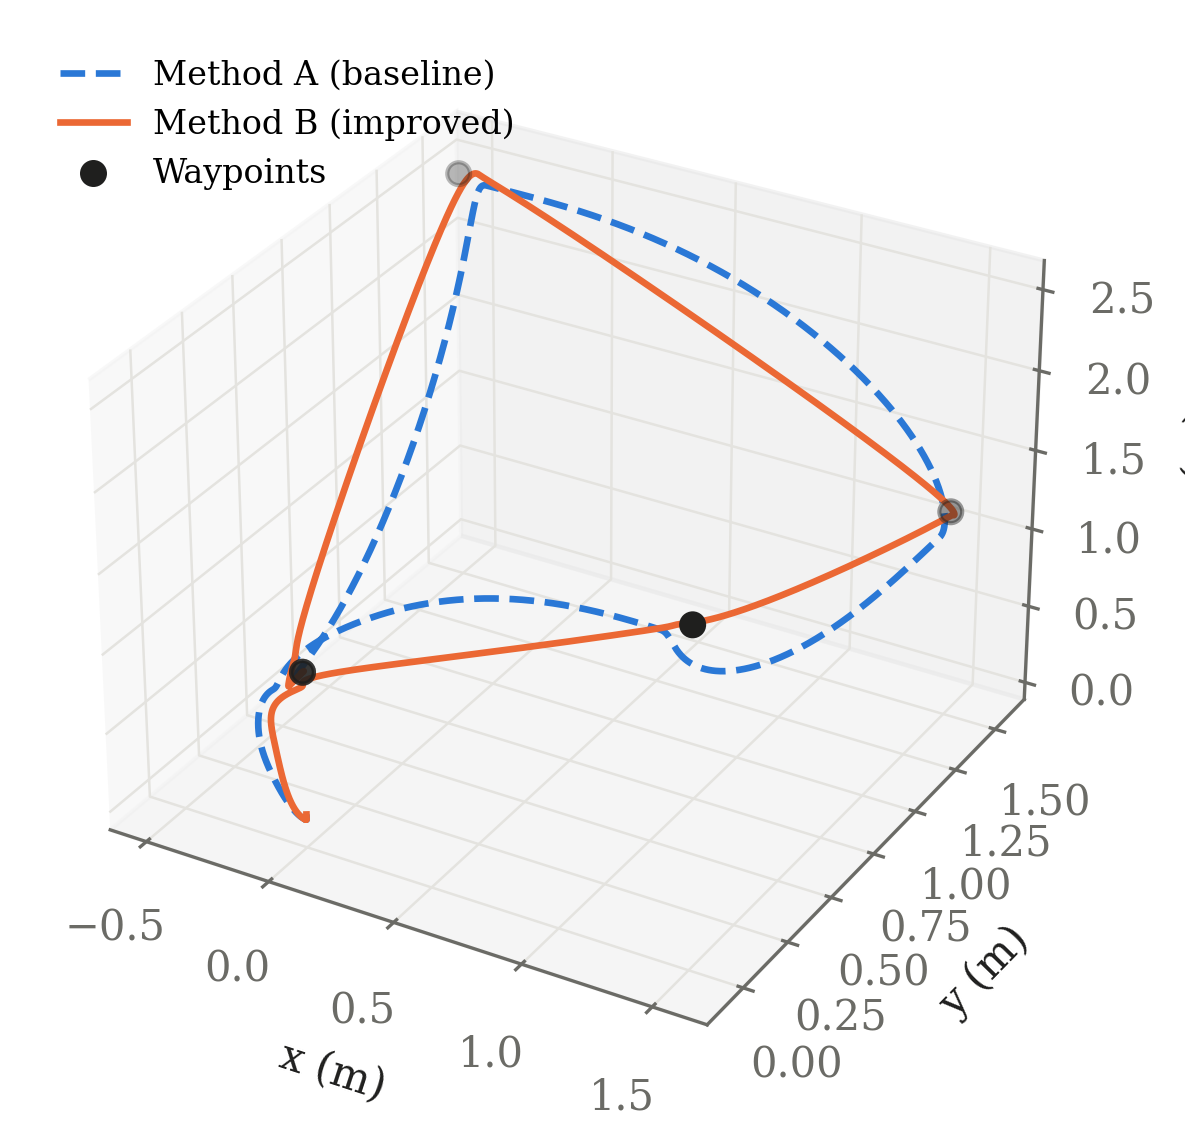
\includegraphics[width=0.44\linewidth]{fig_e3_3d_path.png}
\caption{E3 3D waypoint mission}
\label{fig:e3}
\end{figure}

\begin{table}[h]
\centering
\caption{Waypoint missions without disturbance (E2, E3)}
\label{tab:e2e3}
\begin{tabular}{|p{8.2cm}|c|c|}
\hline
\textbf{Metric} & \textbf{Method A} & \textbf{Method B} \\ \hline
E2 square: Path RMSE (m) & 0.063 & 0.049 \\ \hline
E2 square: Max path error (m) & 0.109 & 0.080 \\ \hline
E2 square: Mission time (s) & 20.8 & 19.2 \\ \hline
E2 square: Peak tilt (deg) & 11.8 & 8.2 \\ \hline
E2 square: Control effort ((rad/s)$^2$) & 27.1 & 12.1 \\ \hline
E3 3D: Path RMSE (m) & 0.275 & 0.046 \\ \hline
E3 3D: Max path error (m) & 0.542 & 0.068 \\ \hline
E3 3D: Mission time (s) & 20.4 & 18.7 \\ \hline
E3 3D: Peak tilt (deg) & 10.2 & 7.4 \\ \hline
E3 3D: Control effort ((rad/s)$^2$) & 35.2 & 12.6 \\ \hline
\end{tabular}
\end{table}


\subsection{E4: crosswind}
From $t = 8$\,s a 0.3\,N crosswind with 0.15\,N gusts pushes the drone along $+y$ (Figures~\ref{fig:e4path} and \ref{fig:e4}). Method A has no integral action. Its position loop needs a steady error to produce the force that balances the wind, so the drone settles about 0.5\,m downwind of the path. That is outside the 0.2\,m arrival tolerance, so Method A reaches only \R{E4}{baseline}{waypoints_reached} of 5 waypoints and never finishes. It does not crash. Method B's velocity-loop integral builds up a constant tilt into the wind. It reaches all five waypoints in \R{E4}{improved}{mission_time_s}\,s with a path RMSE of \R{E4}{improved}{path_rmse_m}\,m (Table~\ref{tab:e4}). The gusts remain visible in Figure~\ref{fig:e4} as small periodic errors, because the integral can cancel the mean force but not the 4\,s oscillation.

\begin{figure}[H]
\centering
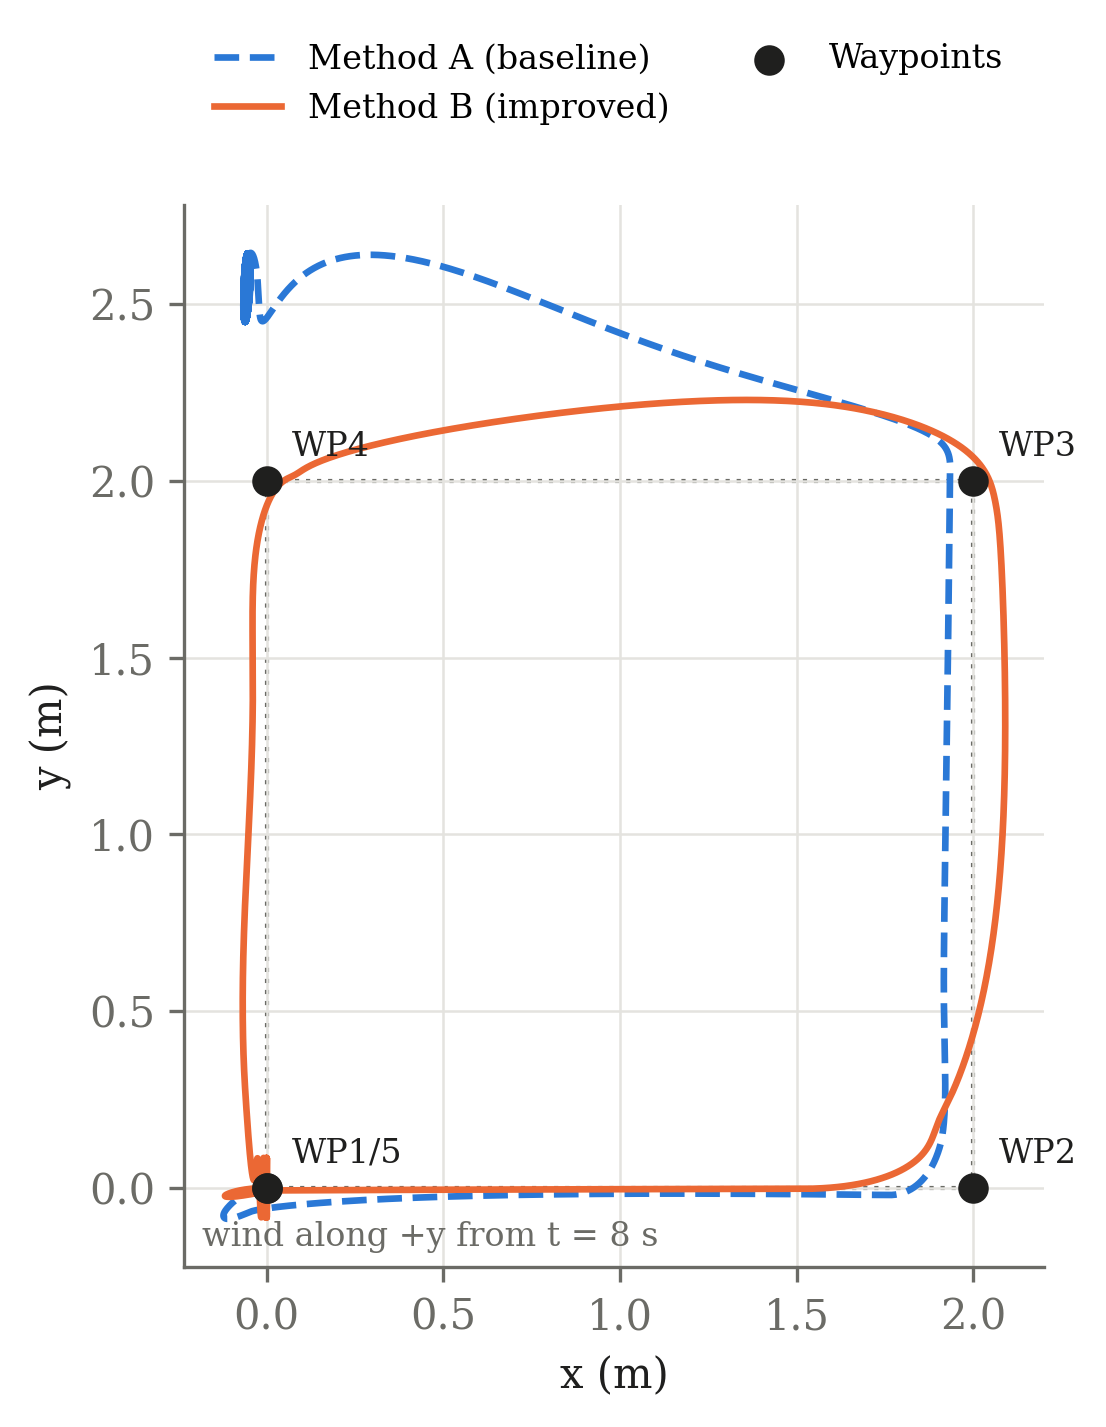
\includegraphics[width=0.45\linewidth]{fig_e4_xy_path.png}
\caption{E4 square mission under crosswind, top view}
\label{fig:e4path}
\end{figure}

\begin{figure}[H]
\centering
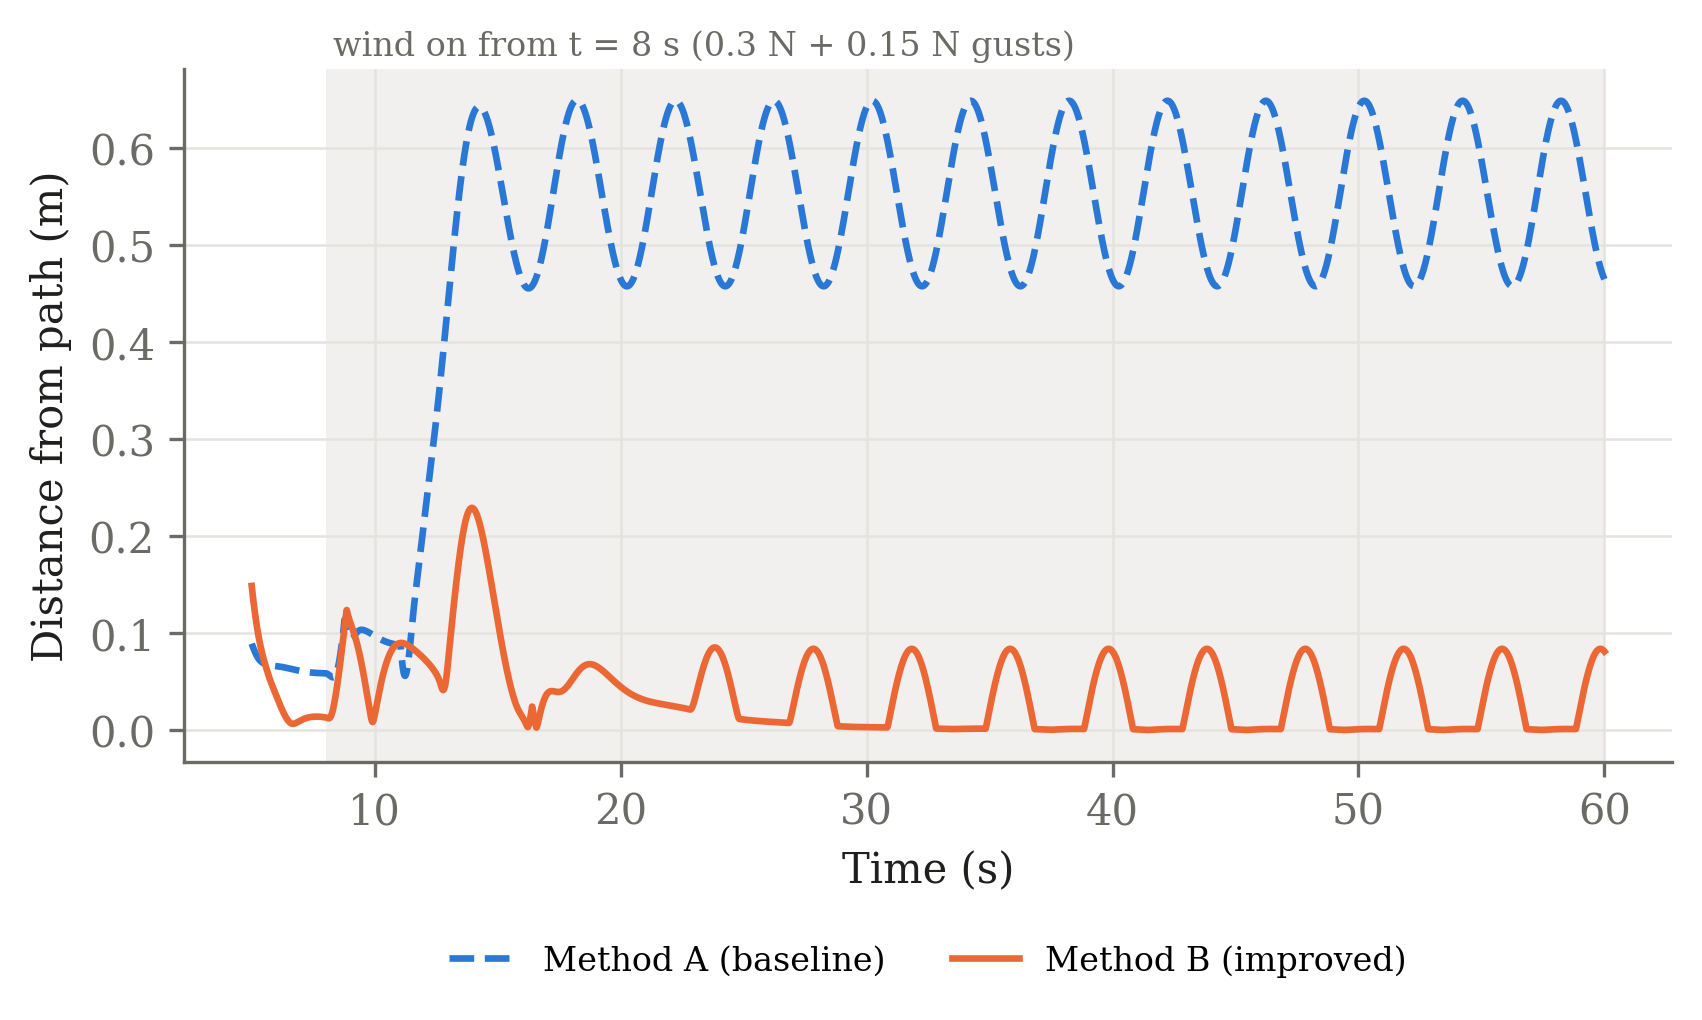
\includegraphics[width=0.62\linewidth]{fig_e4_wind_error.png}
\caption{E4 distance from the planned path over time}
\label{fig:e4}
\end{figure}

\begin{table}[h]
\centering
\caption{Square mission under crosswind (E4)}
\label{tab:e4}
\begin{tabular}{|p{8.2cm}|c|c|}
\hline
\textbf{E4 metric (wind 0.3 N + 0.15 N gusts)} & \textbf{Method A} & \textbf{Method B} \\ \hline
Waypoints reached (of 5) & 3 & 5 \\ \hline
Path RMSE (m) & 0.517 & 0.086 \\ \hline
Max path error (m) & 0.650 & 0.229 \\ \hline
Mission time (s) & -- & 20.0 \\ \hline
Peak tilt (deg) & 13.4 & 11.1 \\ \hline
\end{tabular}
\end{table}


\subsection{E5: sensor noise}
With 5\,cm GPS noise and 0.005\,rad IMU noise, each method flew the square ten times with different random seeds (Table~\ref{tab:e5}, Figure~\ref{fig:e5}). Method B succeeded in \R{E5}{improved}{success} runs, and its path RMSE was almost unchanged from the noise-free case (\R{E5}{improved}{mean_path_rmse_m}\,$\pm$\,\R{E5}{improved}{std_path_rmse_m}\,m against \R{E2}{improved}{path_rmse_m}\,m in E2). Method A succeeded in \R{E5}{baseline}{success} runs and crashed in \R{E5}{baseline}{crash_count}. Its step commands drive the attitude loop hard (Section 9.5), which probably left too little margin for the extra noise in those seeds; we did not log the signals needed to confirm this. This experiment also exposed a real weakness of our first design. With the initial Kalman filter setting every noisy run of both methods crashed, and the estimator had to be retuned (Section 7.4). The noise result therefore depends as much on the shared estimator as on the controller.

\begin{figure}[H]
\centering
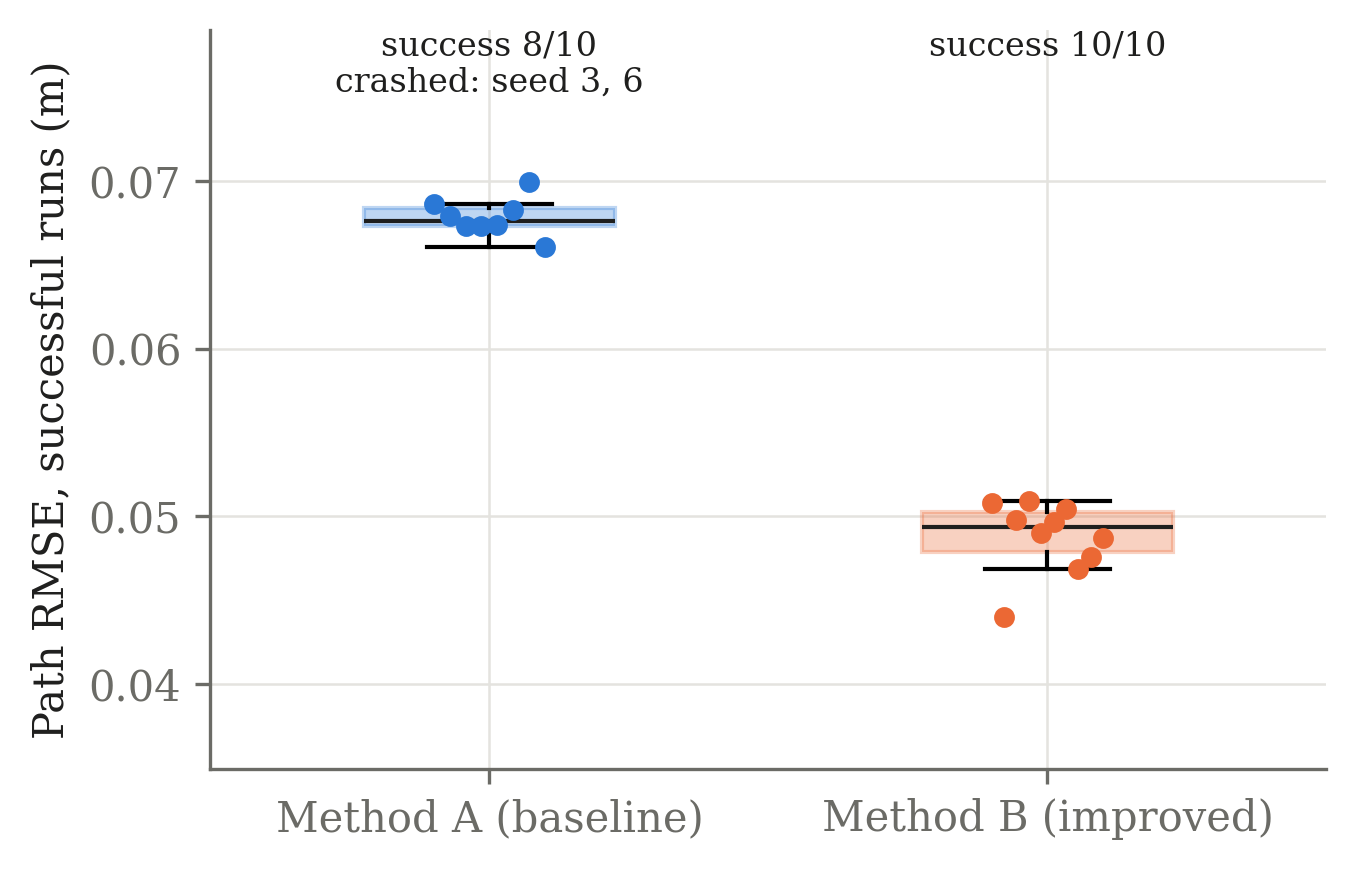
\includegraphics[width=0.48\linewidth]{fig_e5_noise_box.png}
\caption{E5 path RMSE over ten noise seeds}
\label{fig:e5}
\end{figure}

\begin{table}[h]
\centering
\caption{Sensor-noise robustness over ten seeds (E5, mean $\pm$ std of successful runs)}
\label{tab:e5}
\begin{tabular}{|l|c|c|c|c|}
\hline
\textbf{Method} & \textbf{Success} & \textbf{Path RMSE (m)} & \textbf{Mission time (s)} & \textbf{Peak tilt (deg)} \\ \hline
Method A & 8/10 & 0.068 $\pm$ 0.001 & 21.4 $\pm$ 0.3 & 12.6 \\ \hline
Method B & 10/10 & 0.049 $\pm$ 0.002 & 19.5 $\pm$ 0.2 & 9.8 \\ \hline
\end{tabular}
\end{table}


\subsection{E6: roll-gain sensitivity}
The roll proportional gain was swept from 15 to 50, the value used in the Webots sample (Table~\ref{tab:e6}, Figure~\ref{fig:e6}). Method A crashed at $K_{p\phi} \in \{$\R{E6}{baseline}{failed_gains}$\}$, including the sample's own value. Method B completed the mission at every gain (no failures). Both methods use the same attitude loop, so the difference comes from the commands it receives. In the single-axis tests the drone flipped at large roll gains. Our interpretation is that step waypoints demand a sudden large tilt, which a stiff roll loop answers with growing oscillation, while the smooth reference keeps the attitude loop in its small-signal range; we did not log the internal signals that would prove this. Method B is thus much less sensitive to how the inner loop is tuned.

\begin{figure}[H]
\centering
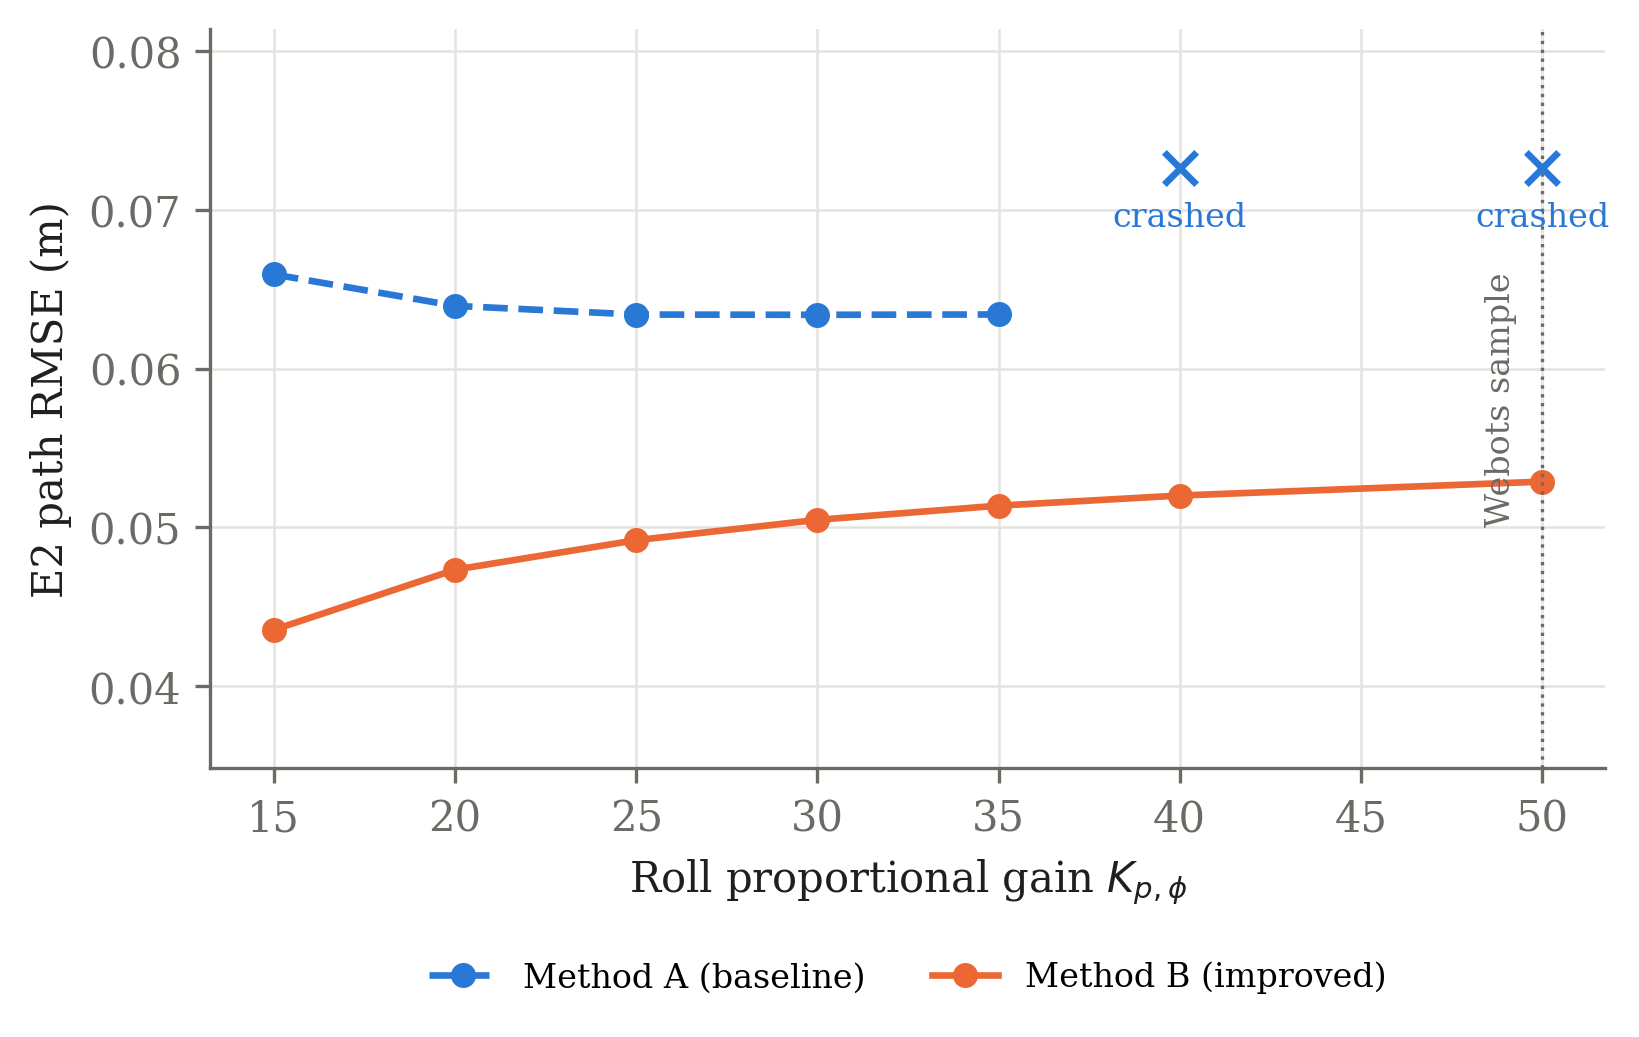
\includegraphics[width=0.65\linewidth]{fig_e6_roll_gain_sweep.png}
\caption{E6 roll-gain sweep: path RMSE of successful runs; crosses mark failed runs}
\label{fig:e6}
\end{figure}

\begin{table}[h]
\centering
\caption{Roll-gain sensitivity on the square mission (E6)}
\label{tab:e6}
\begin{tabular}{|c|c|c|}
\hline
\textbf{Roll $K_p$} & \textbf{Method A} & \textbf{Method B} \\ \hline
15 & success, RMSE 0.066 m & success, RMSE 0.044 m \\ \hline
20 & success, RMSE 0.064 m & success, RMSE 0.047 m \\ \hline
25 & success, RMSE 0.063 m & success, RMSE 0.049 m \\ \hline
30 & success, RMSE 0.063 m & success, RMSE 0.050 m \\ \hline
35 & success, RMSE 0.063 m & success, RMSE 0.051 m \\ \hline
40 & crashed & success, RMSE 0.052 m \\ \hline
50 & crashed & success, RMSE 0.053 m \\ \hline
\end{tabular}
\end{table}


\subsection{What worked and what did not}
\begin{itemize}[itemsep=0pt,topsep=2pt]
\item \textbf{Worked:} measuring the sign conventions first. The pre-project controller had the attitude sign inverted and flipped on every run. Integral action removed the altitude offset and the wind offset. The smooth reference reduced tilt and control effort and made the system tolerant of the roll gain.
\item \textbf{Did not work at first:} the sample's roll gain of 50 was unstable for larger tilt; Method B's first take-off crashed because the reference ignored the climb speed; and the first estimator setting failed under noise. Each failure is recorded in the tuning log, and each fix is described in Section 7.
\item \textbf{Limits:} the simulator has no motor delay, battery sag or ground effect; wind is a force, not airflow; and results are for one drone model and missions of a few metres. Method B also rises more slowly than Method A, because of its smooth reference.
\end{itemize}
